
\begingroup

\definecolor{bloomEdge}{HTML}{718096}
\definecolor{bloomInk}{HTML}{172536}
\definecolor{bloomDeployment}{HTML}{14D2CA}
\definecolor{bloomPool}{HTML}{C6B83F}
\definecolor{bloomFunction}{HTML}{5FC5CE}
\definecolor{bloomAction}{HTML}{CFE5FF}
\definecolor{bloomReserve}{HTML}{FF8069}
\definecolor{bloomContract}{HTML}{E9CFE8}
\definecolor{bloomToken}{HTML}{18D9C2}
\definecolor{bloomFamily}{HTML}{D4C28D}
\definecolor{bloomChain}{HTML}{A5D9FD}

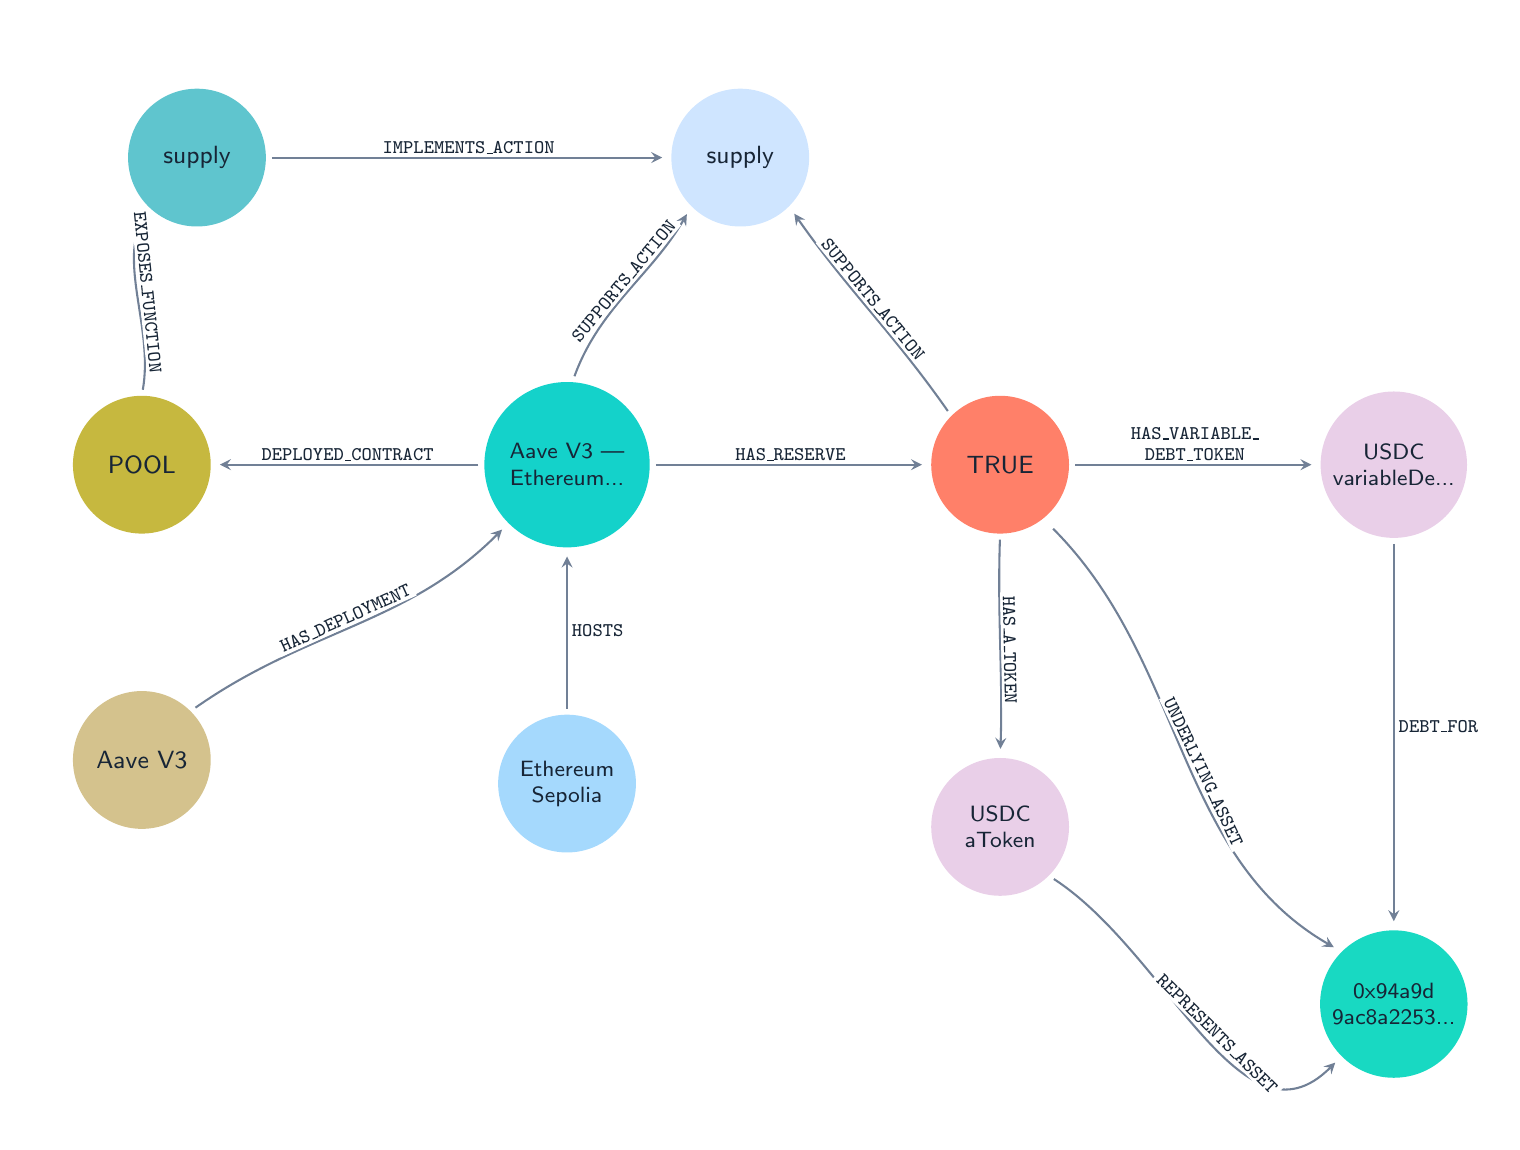
\begin{tikzpicture}[
  >=stealth,
  entity/.style={
    circle,
    draw=none,
    text=bloomInk,
    minimum size=17.5mm,
    inner sep=2.5pt,
    align=center,
    font=\sffamily\fontsize{8.8}{10.1}\selectfont
  },
  compact/.style={
    entity,
    font=\sffamily\fontsize{8.1}{9.4}\selectfont
  },
  main/.style={
    entity,
    minimum size=21mm,
    font=\sffamily\fontsize{8.3}{9.7}\selectfont
  },
  link/.style={
    ->,
    draw=bloomEdge,
    line width=0.75pt,
    shorten <=2pt,
    shorten >=3.1pt
  },
  relation/.style={
    fill=white,
    text=bloomInk,
    align=center,
    inner xsep=1.4pt,
    inner ysep=1pt,
    font=\ttfamily\fontsize{6.7}{7.7}\selectfont
  }
]

% Consistent drawing area
\path[use as bounding box]
  (-7.55,-5.25) rectangle (11.05,8.65);

% --------------------------------------------------
% Graph nodes
% --------------------------------------------------

\node[entity,fill=bloomFunction]
  (fn) at (-5.4,7.0)
  {supply};

\node[entity,fill=bloomAction]
  (action) at (1.5,7.0)
  {supply};

\node[entity,fill=bloomPool]
  (pool) at (-6.1,3.1)
  {POOL};

\node[main,fill=bloomDeployment]
  (deployment) at (-0.7,3.1)
  {Aave V3 ---\\Ethereum...};

\node[entity,fill=bloomReserve]
  (reserve) at (4.8,3.1)
  {TRUE};

\node[compact,fill=bloomContract]
  (debt) at (9.8,3.1)
  {USDC\\variableDe...};

\node[entity,fill=bloomFamily]
  (family) at (-6.1,-0.65)
  {Aave V3};

\node[compact,fill=bloomChain]
  (chain) at (-0.7,-0.95)
  {Ethereum\\Sepolia};

\node[compact,fill=bloomContract]
  (atoken) at (4.8,-1.5)
  {USDC\\aToken};

\node[compact,fill=bloomToken]
  (token) at (9.8,-3.75)
  {0x94a9d\\9ac8a2253...};

% --------------------------------------------------
% p1: Protocol family -> deployment
% --------------------------------------------------

\draw[link]
  (family.north east)
  to[out=35,in=225]
  node[relation,sloped,above,pos=0.48]
    {HAS\_DEPLOYMENT}
  (deployment.south west);

% --------------------------------------------------
% p2: Chain -> deployment
% --------------------------------------------------

\draw[link]
  (chain.north) --
  node[relation,right,pos=0.50]
    {HOSTS}
  (deployment.south);

% --------------------------------------------------
% p3: Deployment -> reserve -> token
% --------------------------------------------------

\draw[link]
  (deployment.east) --
  node[relation,above,pos=0.50]
    {HAS\_RESERVE}
  (reserve.west);

\draw[link]
  ([yshift=-4pt]reserve.south east)
  to[out=-45,in=150,looseness=0.95]
  node[relation,sloped,above,pos=0.55]
    {UNDERLYING\_ASSET}
  (token.north west);

% --------------------------------------------------
% p4: Deployment -> Pool -> Function -> Action
% --------------------------------------------------

\draw[link]
  (deployment.west) --
  node[relation,above,pos=0.50]
    {DEPLOYED\_CONTRACT}
  (pool.east);

\draw[link]
  (pool.north)
  to[out=80,in=245,looseness=0.90]
  node[relation,sloped,above,pos=0.53]
    {EXPOSES\_FUNCTION}
  (fn.south west);

\draw[link]
  (fn.east) --
  node[relation,above,pos=0.50]
    {IMPLEMENTS\_ACTION}
  (action.west);

% --------------------------------------------------
% p5: Deployment -> Action
% --------------------------------------------------

\draw[link]
  ([xshift=2pt]deployment.north)
  to[out=70,in=240,looseness=0.95]
  node[relation,sloped,above,pos=0.53]
    {SUPPORTS\_ACTION}
  (action.south west);

% --------------------------------------------------
% p6: Reserve -> Action
% --------------------------------------------------

\draw[link]
  (reserve.north west)
  to[out=125,in=305,looseness=0.98]
  node[relation,sloped,above,pos=0.53]
    {SUPPORTS\_ACTION}
  (action.south east);

% --------------------------------------------------
% p7: Reserve -> aToken -> underlying token
% --------------------------------------------------

\draw[link]
  (reserve.south)
  to[out=-92,in=88,looseness=0.92]
  node[relation,sloped,above,pos=0.52]
    {HAS\_A\_TOKEN}
  (atoken.north);

\draw[link]
  (atoken.south east)
  to[out=-33,in=225,looseness=1.05]
  node[relation,sloped,above,pos=0.53]
    {REPRESENTS\_ASSET}
  (token.south west);

% --------------------------------------------------
% p8: Reserve -> variable-debt token -> token
% --------------------------------------------------

\draw[link]
  (reserve.east) --
  node[relation,above,pos=0.50]
    {HAS\_VARIABLE\_\\DEBT\_TOKEN}
  (debt.west);

\draw[link]
  (debt.south) --
  node[relation,right,pos=0.48]
    {DEBT\_FOR}
  (token.north);

\end{tikzpicture}
\endgroup
